\documentclass{interact}
%% International Journal of Remote Sensing submission.
%% Taylor & Francis Interact layout class (v1.05), single column for review.
\usepackage{graphicx}
\usepackage{amsmath,amssymb}
\usepackage{array}
\usepackage{xcolor}
\usepackage{url}
\usepackage[authoryear,round]{natbib}
\bibpunct{(}{)}{;}{a}{}{,}
\graphicspath{{figures/}{../figures/}}
\newlength{\tblavail}
%% Floats may take a page top or a float page, never a page bottom: bottom
%% placement let a figure and a table collide, which drew the figure outside the
%% text block. The publisher redoes the page make-up at typesetting anyway.
\usepackage{float}
%% Tighten the reference list: the class default of 1em between 19 entries
%% spills a few lines onto a nearly empty final page.
\setlength{\bibsep}{0.35em}

\begin{document}

\articletype{Research Article}

\title{Protocol choices rival method differences in an audit of 170 remote sensing super-resolution runs}

%% AUTHOR-BEGIN
\author{\name{Zhengyang Chen\textsuperscript{a}\thanks{Email: 18392366572@163.com.
    ORCID: 0009-0003-3310-8077}
  and Dawei Liu\textsuperscript{a}\thanks{*CONTACT Dawei Liu. Email: wjmicheal@163.com}}
\affil{\textsuperscript{a}Engineering University of PAP, Xi'an 710086, China}}
%% AUTHOR-END

\maketitle

\begin{abstract}
Remote sensing super-resolution papers routinely advertise gains as a single number, such as a 0.1 dB gain over the state of the art. Those numbers rest on protocol choices that are rarely reported: which images form the test set, how per-image metrics are aggregated, how many seeds are run, and which baseline convention defines the endpoint. We audit these choices on 170 existing runs spanning four benchmarks, reusing stored per-image artifacts and training nothing. The pool is one laboratory's log, built from three standard architectures plus variants within a single model family, which bounds how far the result generalises. A path-level check confirms identical image sets within each benchmark. Across 327 method pairs, 34.2\% reverse sign between seeds and 65.4\% have an effect smaller than the reference method's seed-to-seed standard deviation, whose median is 0.088 dB against method effects of 0.018 to 0.039 dB. Aggregation and metric choices reorder the ranking in every benchmark, and on the smallest benchmark it crosses method families. A survey of 35 papers from 2026, with 18 full texts retrieved, finds that 7 state a verifiable dB gain and that no abstract mentions seeds, variance, or statistical testing. We close with a seven-item scorecard.
\end{abstract}

\begin{keywords}

\end{keywords}

\noindent\small Word count: 6,218 (main text, excluding abstract,
references and declarations).



\section{Introduction}\label{sec:introduction}

\subsection{The leaderboard rests on unreported choices}\label{sec:unreported}

A reader who wants to decide which super-resolution method to deploy has, in practice, one instrument, namely the ranking published in the paper. That ranking is the output of a pipeline whose steps are individually mundane and collectively decisive. Someone chose the test images. Someone chose PSNR rather than SSIM as the headline number, and chose the mean rather than the median to collapse one number per image into one number per method. Someone chose which baseline checkpoint counts as the baseline. Someone ran the training once, or three times, and reported whichever summary they preferred. Each choice is defensible. Together they determine who wins.

The RS-SR literature reports the ranking and, with few exceptions, omits the choices. Our survey of 35 papers from 2026 finds that no abstract mentions training seeds, variance, or statistical testing. Only four abstracts mention the aggregation convention at all. A reader who wants to know whether a ``+0.1 dB'' claim would survive a rerun with a different random seed has nowhere to look.

The stakes are higher in remote sensing than in generic image restoration, for two reasons. The benchmarks that the field uses most are small, with WHU-RS19 holding 101 test images and UCMerced holding 210, so a per-image statistic is estimated from a short sample. The applications that consume the resulting rankings, from urban impervious-surface mapping to crop monitoring to disaster response, are downstream of a land-cover classifier or a change detector, and a method that wins a benchmark by a fraction of a decibel may not win the application. Both factors push the same way, toward a ranking that is more fragile than its presentation suggests.

\subsection{Opening evidence: a well-documented paper that still ranks by mean}\label{sec:opening}

We begin with a case that requires no reproduction on our part. SpectralSR-Bench (Sensors, 2026) is the only paper in our sample that reports \texttt{mean $\pm$ std} in every table. On disclosure practice it belongs to the best tier we found. Its own reported numbers, however, show that in 8 of 10 adjacent method comparisons the difference in mean PSNR is smaller than the reported per-image standard deviation (Table\textasciitilde{}\ref{tab:srbench}).

\begin{table}[tbp]
\centering
\footnotesize
\setlength{\tabcolsep}{3pt}
\setlength{\tblavail}{\dimexpr\textwidth-10\tabcolsep\relax}
\begin{tabular}{ccccc}
\hline
Method A & Method B & $\Delta$PSNR (dB) & max std (dB) & $\Delta$ / std \\
\hline
FSRCNN ($\times$2) & SRCNN ($\times$2) & 0.38 & 2.20 & 0.17 \\
SRCNN ($\times$2) & SRCNN ($\times$2$\rightarrow$$\times$4) & 3.50 & 2.20 & 1.59 \\
SRCNN ($\times$2$\rightarrow$$\times$4) & SRCNN ($\times$2$\rightarrow$$\times$4$\rightarrow$$\times$8) & 1.45 & 2.20 & 0.66 \\
Bicubic ($\times$2) & Bilinear ($\times$2) & 0.50 & 3.53 & 0.14 \\
Bilinear ($\times$2) & Bicubic ($\times$4) & 1.79 & 3.66 & 0.49 \\
Bicubic ($\times$4) & Bilinear ($\times$4) & 0.42 & 3.66 & 0.11 \\
Bilinear ($\times$4) & Bicubic ($\times$8) & 1.88 & 3.65 & 0.52 \\
Bicubic ($\times$8) & Bilinear ($\times$8) & 0.41 & 3.65 & 0.11 \\
SinSR ($\times$4) & ResShift ($\times$4) & 0.96 & 2.44 & 0.39 \\
ResShift ($\times$4) & SR3 ($\times$8) & 16.11 & 14.80 & 1.09 \\
\hline
\end{tabular}
\caption{Adjacent-pair comparison in SpectralSR-Bench, using the paper's own reported statistics.}\label{tab:srbench}
\end{table}

The \texttt{std} column is the larger of the two reported per-image standard deviations. The last column is the ratio of the mean difference to that dispersion. Eight of the ten ratios are below 1, so the ranking is not resolvable from the reported statistics. The two pairs that do clear the dispersion involve a large change of operating regime, a three-step cascade and a diffusion method near failure. The \texttt{std} here is a per-image dispersion across 50 images, not a seed-to-seed variance, so Table\textasciitilde{}\ref{tab:srbench} speaks to data dispersion only. It is also the one case in the survey where the decisive evidence comes from a paper's own reported numbers, with no recomputation on our part.

The paper discloses dispersion and then ranks by the mean anyway. It did more than its peers, and the conventions of the field still left the decisive comparison ambiguous. When the per-image spread exceeds the gap between methods, a mean-only ranking carries information the reader cannot evaluate.

This case sets the terms of the paper. We argue that the ranking procedure is under-specified, and we measure what that under-specification costs on data where we can control every choice.

\subsection{What existing evaluation critiques address}\label{sec:prior}

Recent work has made evaluation itself an object of study, and each contribution answers a different question from ours.

GeoSR-Bench shows that PSNR improvements correlate weakly, and sometimes negatively, with downstream task performance. SR-Prominence shows that 48.2\% of annotated artifacts go unnoticed by human observers, and that no-reference IQA fails to generalize across datasets. LL-Bench shows that image quality assessment models correlate weakly with human pairwise preferences across 16 tasks. These works ask whether the metric is trustworthy.

NTIRE 2026 addresses protocol ambiguity by fixing it. A 4-pixel border is excluded, all calculation is restricted to the Y channel, and eight metrics are defined precisely. The organizers' score for the infrared track, \texttt{Score = PSNR + 20 $\times$ SSIM}, amplifies SSIM by a factor of 20 relative to PSNR, so that 0.01 SSIM contributes the same as 0.2 dB. This is a gain for reproducibility, because the rule is stated. It is also, in the same breath, an acknowledgment that the weighting rule determines the meaning of the ranking. A change in that factor reorders competitors.

The question these works leave open is the one we take up. Holding the metric fixed and holding the test images fixed, does the ranking stay the same when the protocol choices change. For a given set of methods, how often does swapping the aggregation rule, or the random seed, or the endpoint convention, change who is on top.

\subsection{Contributions}\label{sec:contributions}

We make four contributions.

\textbf{C1. A zero-training audit protocol.} We audit 170 existing runs across four standard benchmarks by reading their per-image evaluation artifacts. No model is retrained. The protocol applies to any SR evaluation that has retained per-image results, which is the common case for a laboratory's own experiment logs.

\textbf{C2. A measurement of the protocol against the effect it is used to rank.} Across 327 method pairs, 34.2\% reverse sign between training seeds and 65.4\% show an effect smaller than the reference method's seed noise. Counting only the pairs whose statistic is assessable, the below-noise fraction ranges from 63.4\% to 70.8\% across three defensible reference conventions, and we report the full range. The seed-to-seed standard deviation has a median of 0.088 dB against method effects of 0.018 to 0.039 dB, so the protocol dominates the quantity being ranked. Aggregation and metric choices reorder the ranking in every benchmark, which follows from that ratio rather than standing as an independent finding. On the smallest benchmark the reordering crosses method families.

\textbf{C3. A report-practice survey.} We code 35 papers on disclosure of aggregation, seeds, and test-set composition. The abstract-level count for seed disclosure is zero. Retrieving 18 full texts raises it to four. The difference between the two counts governs how the whole survey has to be read.

\textbf{C4. A seven-item scorecard.} Each audit finding maps to one check a reader can apply to a published paper, listed in Section\textasciitilde{}\ref{sec:scorecard}.

The remainder of the paper is organized as follows. Section\textasciitilde{}\ref{sec:related} places the audit against related work. Section\textasciitilde{}\ref{sec:methods} specifies the audit design and the pairing rule. Section\textasciitilde{}\ref{sec:results} reports the controlled audit of 170 runs. Section\textasciitilde{}\ref{sec:survey} reports the survey of 35 published papers. Section\textasciitilde{}\ref{sec:scorecard} states the scorecard. Section\textasciitilde{}\ref{sec:discussion} discusses the consequences for authors, reviewers, and editors. Section\textasciitilde{}\ref{sec:discussion}I lists the limitations, and Section\textasciitilde{}\ref{sec:conclusion} concludes.

\section{Related work}\label{sec:related}

\subsection{Metric trustworthiness}\label{sec:metric}

A line of work asks whether the numbers a paper reports correspond to what a human would see \citep{wang2004,blau2018}. LL-Bench \citep{liu2026a} evaluates image quality assessment models against 152,020 human pairwise preferences over 2,469 images and 16 tasks, and finds weak correlation with human judgment. SR-Prominence \citep{molodetskikh2026} reports that 48.2\% of the artifacts its annotators mark are not noticed by viewers, and that no-reference IQA metrics fail to transfer across datasets. Both conclusions concern the metric's validity as a proxy for perceived quality.

Our audit keeps the metric fixed and varies the protocol around it. We do not ask whether PSNR measures quality. We ask whether a ranking built on PSNR is stable when the aggregation or the seed changes. The two questions are independent. A perfectly valid metric can still yield an unstable ranking if the aggregation rule is left free.

\subsection{Downstream correlation}\label{sec:downstream}

GeoSR-Bench \citep{li2026} trains downstream predictors of land-surface variables from super-resolved inputs and finds that PSNR gains do not reliably translate into downstream gains, and in some settings reverse. This is an argument for evaluating on the downstream task rather than on reconstruction fidelity.

Our scope is narrower and orthogonal. We do not evaluate any downstream task. We examine the internal consistency of the reconstruction evaluation itself, on the premise that a downstream comparison inherits any instability present upstream.

\subsection{Protocol standardization}\label{sec:standard}

Competition organizers confront ambiguity directly by fixing it. NTIRE 2026 \citep{chen2026}, \citep{liu2026b} fixes the evaluation region, the color channel, and the metric set, and publishes a weighted score. The choice to weight SSIM by 20 relative to PSNR is a protocol decision made explicit. Its existence is the clearest available evidence that protocol decisions change rankings, since a decision that did not matter would not need to be published and defended.

We differ in direction. Where the organizers unify the protocol so that a single ranking is well defined, we ask how much a ranking moves when the protocol is allowed to vary across the range of defensible options. The NTIRE score tells us what happens under one convention. Our audit reports the spread across conventions.

\subsection{Cross-method fairness}\label{sec:fairness}

SpectralSR-Bench \citep{shokoohi2026} evaluates CNN, GAN, diffusion, and classical methods under a single reproducible pipeline with per-image records. Its contribution is fairness along the method axis, in that every method is measured the same way. One-step diffusion methods such as ORDiffSR \citep{tang2026a} extend the same axis to a newer method family, and their inclusion makes the aggregation question sharper, since a diffusion model and a convolutional model can differ substantially in the shape of their per-image error distribution even when their mean PSNR is close.

We vary along a different axis, holding the method set fixed and changing the measurement convention. The two are complementary. Fairness across methods is necessary for a meaningful ranking. Stability across conventions is necessary for a ranking to survive being read by someone who would have chosen differently.

\subsection{Statistical reporting norms}\label{sec:reporting}

Psychology and natural language processing have established reporting conventions \citep{reimers2017,bouthillier2021}, namely report effect sizes with confidence intervals, run multiple seeds, and prefer equivalence testing to null-hypothesis significance when the claim is that there is no difference. RS-SR has no such norm. Our survey quantifies the gap, and the scorecard in Section\textasciitilde{}\ref{sec:scorecard} adapts these conventions to the specific failure modes we measure.

\subsection{Benchmark scale in remote sensing}\label{sec:scale}

The benchmarks used in this audit carry between 101 and 1000 test images. The small end of that range is typical for remote sensing scene and reconstruction benchmarks, because the underlying acquisitions are expensive and the ground truth requires either very high resolution reference imagery or a physical model. A recent survey of remote sensing foundation models \citep{hong2026} notes that labeled remote sensing data are scarce and costly and that computational efficiency remains a standing challenge. A third consideration belongs beside those two, namely that the statistical resolution of the benchmark itself bounds the resolution of any comparison made on it.

\section{Materials and methods}\label{sec:methods}

\subsection{Data and assets}\label{sec:assets}

The audit reads 170 runs, each of which produced a \texttt{test\_\allowbreak per\_\allowbreak image.jsonl} record with one line per test image holding \texttt{path}, \texttt{psnr}, \texttt{ssim}, \texttt{ergas}, \texttt{sam}, and \texttt{lpips}. The runs span four standard benchmarks, AID (46 runs), RSSCN7 (39), UCMerced (39), and WHU-RS19 (36) \citep{xia2017,zou2015,yang2013,dai2011}. Ten further runs carry no dataset tag and are excluded from all per-benchmark statistics. Test-set sizes are 1000 images for AID, 281 for RSSCN7, 210 for UCMerced, and 101 for WHU-RS19. All four benchmarks are public and are widely used for RS-SR in the aerial and satellite scene setting. The pool is one laboratory's experiment log rather than a sample of published methods. Counting each run name after removing the seed and dataset suffixes gives 20 distinct entries on AID, 17 on RSSCN7, 17 on UCMerced, and 14 on WHU-RS19. Only three of those entries are independent standard architectures, namely a lightweight CNN, a small residual-channel-attention network \citep{zhang2018}, and a 32-channel feature-enhancement network. The lineage these draw on runs from SRCNN \citep{dong2016} through EDSR \citep{lim2017} and RCAN to transformer models such as SwinIR \citep{liang2021}. The remainder are variants within a single model family that differ by one loss weight or one architectural component. The composition bounds what the audit can claim and is carried through the abstract and the limitations.

Every run predates this study. We train nothing. The audit is a re-reading of stored artifacts, which is what makes it cheap and what makes it applicable to any laboratory's existing logs.

\subsection{Four audit lines}\label{sec:lines}

Line B holds the images and methods fixed and varies only the aggregation or the metric. Lines C and D hold the methods and the aggregation fixed and vary only the seed. Line A removes a confound that would invalidate both. Line E tests the pipeline against a comparison whose published value is known.

\subsection{Pairing discipline and a grouping bug}\label{sec:pairing}

We preregistered one rule for the pairing logic, namely that only runs whose names carry an explicit \texttt{\_\allowbreak s20xx} seed suffix participate in method pairing. Runs without a seed suffix are excluded. Of the 170 runs, 160 carry a dataset tag, and 144 of those also carry a seed suffix and enter the pairing. The remaining 26 are set aside, comprising 16 tagged runs without a seed suffix and 10 runs with no dataset tag.

Our first implementation violated this rule, and the error is worth reporting in full. The first version of the effect-versus-noise script grouped the seed-less run \texttt{stage2\_\allowbreak aid\_\allowbreak edge\_\allowbreak deep\_\allowbreak fuse} into the same method family as \texttt{base\_\allowbreak ssm\_\allowbreak aid\_\allowbreak s2026/2027/2028} and paired them seed by seed. The pairing was misaligned, and the script reported $\Delta$ = $-$0.1008 dB, a sign reversal against the published result. We briefly read this as evidence of an error in the original paper.

It was a bug in our grouping function. The seed-less run had no seed to match, so the pairing loop attached it to whichever seed happened to occupy the same position. After restricting pairing to seed-suffixed runs, the same comparison returned +0.0849, +0.1272, and +0.0744 dB across the three seeds, matching the published values to the digit.

A sign-reversed major finding is more likely to be a bug in the audit script than a discovery about the audited work. Line E enforces this, and Section\textasciitilde{}\ref{sec:anchor} gives the demonstration: an audit must reproduce a result that is known to hold before it reports that someone else's does not.

\subsection{Coding scheme and evidence tiers}\label{sec:coding}

We surveyed 35 papers on RS-SR and its evaluation, published mainly in 2026, drawn from arXiv, MDPI, Nature Scientific Reports, IEEE, and Elsevier venues. Each paper was coded on whether it discloses its aggregation convention (R2), its training-seed count (R3), and its test-set composition (R5). Not every paper was readable in full, so each coded field carries an evidence tier. Tier A means the field is stated in the abstract or a retrieved fragment. Tier B means a portion of the body text supports it. Tier C means the field could not be confirmed without the full text.

A tier-C code means not yet confirmed, not absent, and that distinction decides whether the survey can claim a field is missing at all, as Section\textasciitilde{}\ref{sec:fulltext} shows.

We retrieved full texts for 18 of the 35 papers, using the publisher's open-access channel where available and the publisher's own PDF endpoint otherwise. Eleven of the remaining papers are closed access at the publisher, confirmed against OpenAlex metadata, and six have no article PDF at all.

Four of the 35 items are not standalone published articles, namely one duplicate record, one competition leaderboard, and two entries whose only source was a non-peer-reviewed page. Every percentage in this section is reported against the full 35-item sample. A reader who prefers a denominator restricted to published articles should divide by 31 instead, and the item-by-item composition is recorded in the data repository.

\section{Results}\label{sec:results}

The method pool is one laboratory's log, built from three standard architectures plus variants of a single model family (Methods). The results below therefore measure how far protocol choices can move a ranking within that pool, and the seed-noise analysis bounds how much of the movement is resolvable at all.

\subsection{Line A: the test sets are identical}\label{sec:testsets}

All 170 runs pass. Within each benchmark, the set of image paths is identical across every run, the Jaccard index is 1.0, the recorded size matches the split file, and no metric value is missing or NaN.

The instability reported below is not a test-set artifact. Whatever moves a ranking here, it is not the images.

\subsection{Line B: aggregation reorders the ranking}\label{sec:champion}

\begin{table}[tbp]
\centering
\footnotesize
\setlength{\tabcolsep}{3pt}
\setlength{\tblavail}{\dimexpr\textwidth-10\tabcolsep\relax}
\begin{tabular}{ccccc}
\hline
Convention & AID (46) & RSSCN7 (39) & UCMerced (39) & WHU-RS19 (36) \\
\hline
\texttt{psnr\_\allowbreak mean} (reference) & 1.000 & 1.000 & 1.000 & 1.000 \\
\texttt{psnr\_\allowbreak median} & \textbf{0.882} $\times$ & \textbf{0.502} $\times$ & \textbf{0.818} $\times$ & \textbf{0.749} $\times$ \\
\texttt{psnr\_\allowbreak trim10} & 0.979 & 0.987 & 0.996 & 0.934 \\
\texttt{psnr\_\allowbreak trim25} & 0.962 & 0.986 & 0.981 & 0.833 \\
\texttt{ssim\_\allowbreak mean} & 0.868 & \textbf{0.957} $\times$ & 0.747 & 0.807 \\
\texttt{ergas\_\allowbreak mean} & 0.943 & \textbf{0.982} $\times$ & 0.945 & 0.944 \\
\texttt{sam\_\allowbreak mean} & 0.813 & \textbf{0.535} $\times$ & 0.793 & \textbf{0.272} $\times$ \\
\texttt{lpips\_\allowbreak mean} & 0.534 & \textbf{0.894} $\times$ & 0.549 & 0.860 \\
\hline
\end{tabular}
\caption{Rank correlation against mean PSNR, and whether the champion changes.}\label{tab:conventions}
\end{table}

$\times$ marks a convention under which the top-ranked method differs from the \texttt{psnr\_\allowbreak mean} champion.

Table\textasciitilde{}\ref{tab:conventions} reports, for each benchmark, the Spearman rank correlation between the ranking under each of eight conventions and the ranking under mean PSNR, together with whether the top-ranked method changed. Three results stand out.

\textbf{Median aggregation reverses the champion on all four benchmarks.} The median guards against the outlier sensitivity that a small test set invites, and replacing the mean with it changes the top-ranked method on AID, RSSCN7, UCMerced, and WHU-RS19. The rank correlation drops as low as 0.502, on RSSCN7.

\textbf{Trimmed aggregation preserves the ranking.} The 10\% and 25\% trimmed means keep a rank correlation of at least 0.833 with mean PSNR, and mostly above 0.93, across every benchmark. The trimmed mean discards the extremes while retaining the bulk of the distribution, and the ranking is stable under it.

The contrast between the median and the trimmed mean localizes the source. Both are robust aggregators, yet the median reorders and the trimmed mean does not. The difference is that the median depends on the middle order statistics and is sensitive to how the distribution shifts in the center, while the trimmed mean averages the bulk and retains the mean's insensitivity to that shift. The instability therefore lives in the tails and near the center, not in the overall shape. This is an operational diagnostic. When a benchmark's ranking is highly sensitive to the convention, the first thing to inspect is the distribution of the per-image scores, not the choice of metric. One qualification applies to the flip count. The method pool behind these rankings is dominated by variants of a single model family (Methods), so a flip between the top two entries is often a reordering of near-identical variants, which the seed-noise analysis in the next subsection explains. The WHU-RS19 case below is the exception, because there the two candidates belong to different method families, and it is the clearest evidence that the effect is not confined to close variants.

\textbf{On WHU-RS19, switching the metric changes the winner's method family.} The SAM convention carries the lowest rank correlation in the whole study, 0.272, on WHU-RS19. The champion under mean PSNR is a residual-channel-attention network. Under SAM it is a lightweight CNN. The two methods differ not in depth or width but in family, and the benchmark that produces this reversal is the smallest, at 101 test images.

\subsection{Lines C and D: effect size against seed noise}\label{sec:noise}

We pair every two runs of the same benchmark that share a seed and belong to different methods, and compute the mean difference in PSNR over the paired images. Across 327 pairs we record the mean effect, the standard deviation of the per-image differences within each method, and whether the effect keeps its sign across seeds.

The noise comparison depends on which standard deviation serves as the reference, so we report all three definitions.

The strictest rule counts a pair as below the noise only when the effect is smaller than the smaller of the two methods' seed standard deviations, so that both methods are noisier than the effect. That gives 154 of the 243 pairs in which both methods have a defined seed standard deviation, 63.4\%.

The definition we carry through the paper compares the effect against the seed standard deviation of the reference method in each pair, fixed as the first method so that the count is deterministic. That gives 172 of the 263 pairs with a defined reference standard deviation, 65.4\%.

The symmetric definition compares the effect against the larger of the two seed standard deviations and gives 172 of the same 243 pairs, 70.8\%. The three definitions span 63.4\% to 70.8\% and agree on the direction of the finding. We carry the middle one because its reference is explicit, and report all three for a reader who prefers a different convention. Table\textasciitilde{}\ref{tab:effect} collects these counts.

Two conventions govern these denominators, and both matter more than they look. A pair whose two methods share only one seed cannot reverse, so it is excluded from the reversal count rather than scored as consistent, which leaves 243 of the 327 pairs. A pair without a defined reference standard deviation cannot be compared with the noise, so it is excluded from that count rather than scored as not below the noise. Scoring an unassessable pair as a null result would bias both percentages downward, which is the reporting failure this paper is about. The 327 pairs are also not independent, because each method enters many of them, so a binomial interval over 327 would be too narrow. We give 95\% intervals from a cluster bootstrap that resamples methods within each benchmark and weights every pair by the product of its endpoints' multiplicities: 34.2\% of pairs reverse, interval 20.9\% to 49.4\%, and 65.4\% fall below the reference noise, interval 49.3\% to 81.9\%.

\begin{table}[tbp]
\centering
\footnotesize
\setlength{\tabcolsep}{3pt}
\setlength{\tblavail}{\dimexpr\textwidth-4\tabcolsep\relax}
\begin{tabular}{>{\centering\arraybackslash}m{0.640\tblavail}>{\centering\arraybackslash}m{0.330\tblavail}}
\hline
Quantity & Value \\
\hline
Method pairs analyzed & 327 \\
Pairs with two or more shared seeds & 243 \\
Pairs with a defined reference seed sd & 263 \\
Pairs that reverse sign across seeds & \textbf{83 (34.2\%)} of 243 \\
Pairs with $|$effect$|$ below the reference method's seed sd & \textbf{172 (65.4\%)} of 263 \\
Pairs with $|$effect$|$ below the smaller of the two methods' seed sds & 154 (63.4\%) of 243 \\
Pairs with $|$effect$|$ below the larger of the two methods' seed sds & 172 (70.8\%) of 243 \\
Median seed-to-seed standard deviation & \textbf{0.088 dB} (range 0.049 to 0.248) \\
Median method effect & \textbf{0.018 to 0.039 dB} \\
\hline
\end{tabular}
\caption{Effect size against seed noise.}\label{tab:effect}
\end{table}

The seed noise is two to five times the size of the method effect it is supposed to discriminate. One in four method pairs reverses order when the seed changes. Slightly more than half of all pairs show a difference smaller than the noise.

The per-benchmark noise, reported in Supplementary Table S2, follows the test-set size. WHU-RS19, at 101 images, has the largest noise and, at 47.3\%, the highest reversal rate, with 80\% of its pairs falling below the noise. AID, at 1000 images, has the smallest noise. The ordering is monotone in test-set size, with one inversion between AID and RSSCN7 that we attribute to the differing content heterogeneity of the two benchmarks rather than to size alone. Fig.\textasciitilde{}\ref{fig:1} shows this relation.

\begin{figure}[tbp]
\centering
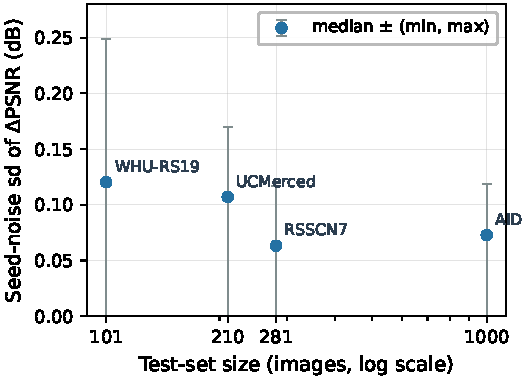
\includegraphics[width=0.55\textwidth]{fig1_noise_vs_testsize.pdf}
\caption{Seed noise against test-set size.}
\label{fig:1}
\end{figure}

The horizontal axis is the number of test images on a logarithmic scale and the vertical axis is the median seed-to-seed standard deviation of the paired per-image PSNR difference in dB. Each marker is one benchmark and the error bars span the minimum to the maximum standard deviation observed for it. The four points are AID (1000 images, 0.0728 dB), RSSCN7 (281, 0.0632 dB), UCMerced (210, 0.1070 dB), and WHU-RS19 (101, 0.1202 dB). A fixed absolute effect, such as the 0.1 dB that RS-SR papers commonly claim, is therefore compared against a smaller noise floor on a large benchmark and a larger one on a small benchmark.

The practical implication is direct. The headline convention in RS-SR, stating that a method exceeds the previous best by 0.1 dB, sits inside the noise band on small benchmarks. On WHU-RS19, a 0.1 dB claim is below the median seed variation. Fig.\textasciitilde{}\ref{fig:2} shows all 327 pairs.

\begin{figure}[tbp]
\centering
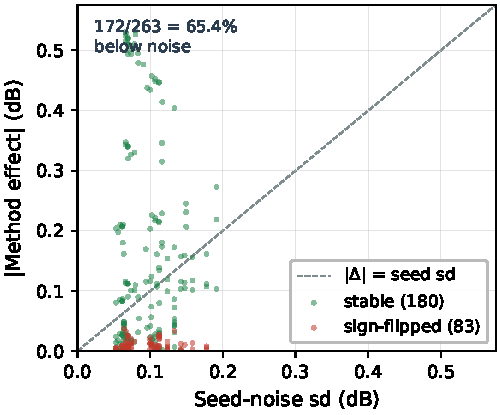
\includegraphics[width=0.55\textwidth]{fig2_effect_vs_noise.pdf}
\caption{Method effect against seed noise, for all 327 pairs.}
\label{fig:2}
\end{figure}

The horizontal axis is the absolute mean paired PSNR difference in dB and the vertical axis is the seed-to-seed standard deviation of that difference in dB. Both axes are logarithmic and a dashed line marks equality. Points above the line have an effect larger than the noise. Points below the line, colored, are the 172 pairs whose difference does not clear the noise floor under the reference-method definition. The cluster near the lower-left corner corresponds to pairs on AID between method variants that differ by a single component, where both the effect and the noise are of order 0.01 dB.

\subsection{Line E: the pipeline reproduces a known result}\label{sec:anchor}

We verify the pipeline against a comparison whose published value is known. We recompute the BSRNet variant B3 against the baseline \texttt{base\_\allowbreak ssm} from the stored per-image artifacts and compare to the published numbers.

The pipeline reproduces both published figures exactly. It also shows that changing only the baseline convention, from the primary endpoint to the legacy one, moves the reported effect by 0.0049 dB, about 5\% of the effect itself. In a context where the median method effect is 0.018 to 0.039 dB, a 5\% shift from a convention change is not negligible. The magnitude is small in absolute terms and decisive in relative terms.

\subsection{Report-practice statistics}\label{sec:survey}

Table\textasciitilde{}\ref{tab:practice} reports the full breakdown.

\begin{table}[tbp]
\centering
\footnotesize
\setlength{\tabcolsep}{3pt}
\setlength{\tblavail}{\dimexpr\textwidth-4\tabcolsep\relax}
\begin{tabular}{>{\centering\arraybackslash}m{0.676\tblavail}>{\centering\arraybackslash}m{0.294\tblavail}}
\hline
Field & Count \\
\hline
State a verifiable specific dB gain & \textbf{7 / 35 (20.0\%)} \\
Qualitative SOTA, absolute PSNR only, or efficiency only & \textbf{28 / 35 (80.0\%)} \\
Provide a code or data link & 5 / 35 (14.3\%) \\
Mention seeds, variance, or a statistical test in the abstract & \textbf{0 / 35 (0.0\%)} \\
Mention the aggregation convention in the abstract & 4 / 35 (11.4\%) \\
Anchor to a downstream task or protocol reproduction & 11 / 35 (31.4\%) \\
Disclose R2 in the body (of 18 full texts) & 8 / 35 \\
Disclose R3 in the body (of 18 full texts) & 4 / 35 \\
Disclose R5 in the body (of 18 full texts) & 15 / 35 \\
\hline
\end{tabular}
\caption{Report practice in 35 papers.}\label{tab:practice}
\end{table}

Four fifths of the surveyed papers do not state a number a reader could check. They report an absolute PSNR, or claim a qualitative improvement over the state of the art, or compare only efficiency. The gain-versus-noise comparison in Section\textasciitilde{}\ref{sec:gains} applies only to the 7 papers that give a number. For the other 28 there is no claim to test.

The abstract-level count for seed disclosure is zero. Not one of the 35 abstracts mentions a seed, a variance, or a statistical test. Only four abstracts mention how the per-image metrics were aggregated.

\subsection{Full texts change the seed count}\label{sec:fulltext}

Retrieving 18 full texts changes the seed-disclosure count from zero to four. The papers that do it are specific.

EORestore-Agent \citep{qi2026} trains seven models that differ only in random seed and averages their predictions at inference. It is the only multiple-seed ensemble in the sample. GeoSR-Bench \citep{li2026} trains its downstream prediction models three times per evaluation case and reports the average over the runs. SFG-SwinSR \citep{hossain2026} fixes the random seed of 42 for shuffling and weight initialization. The infrared track of NTIRE 2026 \citep{chen2026} lists a seed of 42 in a team's table.

These four papers refute the reading that no one in the field uses seeds. They were invisible at the abstract level and visible only in the body.

The finding is about reporting, not practice. RS-SR authors do run seeds. The field's norm simply does not require the count to appear where a reader looks, which is the abstract and the results table. The remedy follows from the diagnosis. If authors were not running seeds, the fix would be to run them, and because some authors run them and omit them, the fix is a reporting standard.

The count of papers that do not report a field is bounded above by the number of full texts retrieved, and we report both counts for every field.

\subsection{Claimed gains against the noise floor}\label{sec:gains}

For the 7 papers that state a verifiable dB gain, we compare the claimed effect to the seed noise measured on the same benchmark in Section\textasciitilde{}\ref{sec:noise}. Where the paper's benchmark is outside our pool, we fall back to the pool-wide median and mark the fallback. Table\textasciitilde{}\ref{tab:gains} lists the seven claims against the noise floor of their own benchmarks.

\begin{table}[tbp]
\centering
\footnotesize
\setlength{\tabcolsep}{3pt}
\setlength{\tblavail}{\dimexpr\textwidth-10\tabcolsep\relax}
\begin{tabular}{>{\centering\arraybackslash}m{0.384\tblavail}>{\centering\arraybackslash}m{0.141\tblavail}>{\centering\arraybackslash}m{0.202\tblavail}>{\centering\arraybackslash}m{0.081\tblavail}>{\centering\arraybackslash}m{0.162\tblavail}}
\hline
Paper & Claimed $\Delta$ & Benchmark (noise source) & $\Delta$ / max sd & Reading \\
\hline
PLAN \citep{patnaik2026} & +0.07 dB & AID (measured) & 0.59 & below noise \\
DBTSR \citep{tang2026b} & +0.12 dB & AID (measured) & 1.01 & marginal \\
JNUN-CA & +0.19 dB & WHU-RS19 (measured) & 0.76 & below noise \\
IR275K \citep{deng2026} & +0.35 dB & infrared (fallback) & 1.41 & marginal \\
AstraMoE-SR \citep{lai2026} & +0.64 dB & DOTA (fallback) & 2.58 & clears noise \\
DFSMamba \citep{yu2026} & +1.07 dB & AID (measured) & 9.02 & clears noise \\
EORestore-Agent \citep{qi2026} & +2.30 dB & Landsat-8 (fallback) & 9.27 & clears noise \\
\hline
\end{tabular}
\caption{Claimed gains against the seed-noise floor.}\label{tab:gains}
\end{table}

JNUN-CA carries no reference number because its bibliographic record could not be completed to the standard required for citation, and the data repository records why.

Two of the seven claims fall below the noise ceiling, and two more sit just above it.

The large gains, 0.64 dB and above, clear the noise by a wide margin and are real. The problem sits in the crowded interval between 0.05 and 0.19 dB, which is exactly where the claim of beating the state of the art by 0.1 dB lives. There, on benchmarks the size of WHU-RS19, the claim and the noise are the same order of magnitude.

\subsection{Positive exemplars}\label{sec:exemplars}

Four papers show that the practices we recommend are already used, just not treated as standard.

GrasslandGAN \citep{noayarasca2026} defines the coefficient of variation as the ratio of standard deviation to mean, classifies variability by it, checks normality, and applies the Kruskal-Wallis test with the H statistic and p-values throughout. It is the only paper in the sample that performs distribution-level stability analysis with a significance test.

THREASURE-Net \citep{kalinicheva2025} reports values as the median with the 25th and 75th percentiles, and applies a Mann-Kendall test. It is one of two papers in the sample that uses a median rather than a mean.

AstraMoE-SR \citep{lai2026} states that its aggregates are area-weighted, and gives the reason for choosing DINO as the primary semantic-fidelity criterion, namely that pixel-wise metrics can be sensitive to nuisances the semantic measure ignores. It discloses both the aggregation and the rationale for the primary metric.

The NTIRE 2026 organizers \citep{chen2026}, \citep{liu2026b} publish a weighted score and state its interpretation, that an SSIM improvement of 0.01 contributes the same as 0.2 dB of PSNR. The organizers made the weighting explicit, which is the clearest available acknowledgment that the weighting rule determines the ranking.

\subsection{Two failure modes with names}\label{sec:failures}

Two cases from the 2026 literature illustrate failure modes worth naming.

\textbf{Conflating fairness with reproducibility.} MLIN-MetaWeight \citep{zhang2026} writes that it ensures fairness and reproducibility by training all models under identical batch sizes and iteration counts. Holding hyperparameters constant makes the comparison fair across methods. It does not make the result reproducible across seeds, which requires repeating the training. The two properties are different, and a reporting standard should not let the first stand in for the second.

\textbf{Zero seed disclosure in a long paper.} SDGAN-SciRep \citep{wang2026} runs to roughly 80,000 characters, reports six or more metrics including PSNR, SSIM, AG, NIQE, FID, and IS, and includes distribution plots. The words seed, three runs, and repeat do not appear. The absence is not a matter of space. It reflects the norm that seed information is not part of what a paper reports.

\subsection{Closed access limits external audit}\label{sec:closed}

Of the 19 papers not retrieved in full, 11 are closed access at the publisher, confirmed against OpenAlex metadata, and 6 have no article PDF. The closed set is spread across Elsevier, IEEE, and ACM.

The implication extends past our survey. A third party cannot perform a reproduction-level audit of the closed portion of the RS-SR literature, because the artifacts are not available. What a reader can access is the paper's own reported metadata, which is the abstract and the tables. This raises the stakes on the reporting norm. Where an external audit is impossible, the paper's self-reported protocol information becomes the only basis on which a reader can judge the ranking.

\subsection{The R1 to R7 reproducibility scorecard}\label{sec:scorecard}

The audit findings reduce to seven checks. Each check names a disclosure whose absence produces a specific failure. Table\textasciitilde{}\ref{tab:scorecard} states each check and the failure its omission produces.

\begin{table}[tbp]
\centering
\footnotesize
\setlength{\tabcolsep}{3pt}
\setlength{\tblavail}{\dimexpr\textwidth-8\tabcolsep\relax}
\begin{tabular}{>{\centering\arraybackslash}m{0.038\tblavail}>{\centering\arraybackslash}m{0.384\tblavail}>{\centering\arraybackslash}m{0.321\tblavail}>{\centering\arraybackslash}m{0.227\tblavail}}
\hline
\# & Check & Failure when omitted & Status in the audit pool \\
\hline
R1 & Is the test-set image list public and identical across runs & Cross-paper comparison is void & Pass in all 170 runs \\
R2 & Is the metric aggregation stated (mean, median, trimmed) & The champion flips under the convention & Not stated in 31/35 papers \\
R3 & Are three or more seeds run, with per-seed direction reported & The 34.2\% reversal rate is invisible & 2 seeds in part of the pool \\
R4 & Is the seed-noise magnitude reported & A reader cannot tell whether $|$$\Delta$$|$ clears the noise & Not reported \\
R5 & Is the baseline convention fixed to one run and endpoint & The effect inflates by 5\% or more & Two conventions used \\
R6 & Is equivalence testing used rather than significance alone & No difference reads as improvement & Used only for final confirmation \\
R7 & Are per-image paired confidence intervals and d\_z reported & Stability is unjudgeable & Not reported \\
\hline
\end{tabular}
\caption{The R1 to R7 scorecard.}\label{tab:scorecard}
\end{table}

The scorecard is meant to be applied to a published paper, producing a profile of which of the seven a paper omits. It applies to competition reports as well as method papers, since both publish rankings.

The checks are ordered by the cost of omission we measured. R2 carries the largest measured effect, since it flips the champion on four of four benchmarks. R3 and R4 together carry the reversal rate and the noise floor. R5 carries the 5\% endpoint shift. R1 is listed first because it is a prerequisite, in that a comparison built on different images is not a comparison.

\section{Discussion}\label{sec:discussion}

\subsection{This is a norm problem, not a capability problem}\label{sec:norm}

The survey contains a demonstration that the recommended practices are achievable. GrasslandGAN performs distribution-level analysis with a significance test. SpectralSR-Bench reports dispersion in every table. THREASURE-Net reports medians and quartiles. These papers are not methodologically exotic. They are ordinary papers that chose to report more.

The gap between what is done and what is standard is therefore not a gap in tooling or skill. It is a gap in what the field asks for. Raising the standard is a matter of reviewers and organizers requiring the disclosure, which is why Section\textasciitilde{}\ref{sec:recommend} gives concrete requirements.

\subsection{What the ranking instability means for remote sensing applications}\label{sec:applications}

A benchmark ranking in RS-SR is not an end in itself. It is a screening instrument for methods that will later be run on real acquisitions, over regions and sensors that the benchmark did not cover. The instability we measure has a specific consequence for that use.

Consider a practitioner who reads the ranking and selects the top method for an urban mapping pipeline. If the gap to the second method is 0.1 dB on a benchmark of 210 images, the selection is not supported by the reported statistic, because the seed-to-seed standard deviation on that benchmark is 0.107 dB. The second method may be equally good, and it may be cheaper, lighter, or more robust to the distribution shift that separates the benchmark from the deployment region. The ranking does not carry the information the practitioner needs.

The failure is asymmetric across benchmark size. On AID, with 1000 test images and a noise floor of 0.0728 dB, a 0.1 dB claim is marginally resolvable. On WHU-RS19, with 101 images and a noise floor of 0.1202 dB, the same claim is inside the noise. A field that reports one number without the noise floor therefore publishes a ranking whose interpretability depends on a property of the benchmark that the ranking does not display.

\subsection{The audit joins a shift already under way}\label{sec:shift}

The evaluation-focused works cited above, from the benchmark critiques to the NTIRE protocol reports, mark a shift of attention toward how super-resolution is measured and not only how well it performs. This paper addresses one gap within that shift, which is ranking stability. The existing critiques establish that metrics are imperfect proxies and that protocols need standardizing. This paper asks how much a ranking moves when the protocol varies within the range of defensible choices, and answers with a measured fraction.

\subsection{Recommendations}\label{sec:recommend}

For authors, three disclosures cover most of the measured risk. State the aggregation convention. State the seed count, or state that a single seed was used and name it. State the seed-noise magnitude, so that a reader can compare it against the claimed effect.

For reviewers and editors, two requirements follow from the audit. When a claimed effect is smaller than the reported seed noise, require an equivalence test rather than a significance test. When the test set is small, below roughly 200 images, require that the cross-seed direction of the ranking be reported, because that is where the reversal rate is highest.

A third requirement applies to the tooling that will enforce the other two. Automated reference resolution has to compare the title as well as the response status. While building the reference list for this survey, one DOI carried in our own pool returned HTTP 200 and resolved to a paper on reinforcement learning in the journal *Engineering*, not to the super-resolution paper it was recorded against. A status-only check accepts that record. The correct record was recovered by querying Crossref with the publisher's article identifier, which returned *UDAMSR Net: An Unsupervised Degradation-Aware Network for Enhancing the Spatial Resolution of Spectral Images for Crop Sensing*. Every other number in this paper comes from an audit pipeline whose pairings were validated against stored per-image path sets rather than identifiers, which is why the mis-resolved DOI left the results untouched. Reference handling needs the same discipline, where a single mis-resolved DOI stays invisible unless the title is checked.

\subsection{Consequences for reading a ranking}\label{sec:reading}

A ranking is a summary of a protocol. When the protocol is published, the ranking can be read as a statement about the methods under that protocol. When the protocol is omitted, and the effect is inside the noise band, the ranking does not distinguish methods. Our measurements give the boundary of that band for the four benchmarks studied, in that a claim below the reported seed standard deviation, on a test set of the sizes considered here, cannot be distinguished from noise by a reader who has only the mean.

\subsection{Limitations}\label{sec:limitations}

\begin{enumerate}
\item The findings from our own pool of 170 runs do not extend to the claim that all RS-SR papers have a 1-in-3 error rate. The 34.2\% reversal figure includes many method pairs on AID that are close variants, and close variants are expected to sit near the noise floor.
\item Only 7 of 35 papers state a verifiable gain, so the gain-versus-noise table is illustrative rather than representative. Of those 7 verifiable claims, 2 fall below the measured noise ceiling on the same benchmark.
\item The seed noise is measured on our own pool. For papers whose benchmarks fall outside it, such as the infrared, DOTA, and Landsat-8 cases, we fall back to the pool-wide median and mark the fallback. Those entries cannot be read as the noise on the paper's own benchmark.
\item The abstract-level count of zero for seed disclosure describes abstracts, not practice. Section\textasciitilde{}\ref{sec:fulltext} shows the count rises to four once full texts are read.
\item Three cited papers carry an evidential boundary. The dispersion SpectralSR-Bench reports is per-image across 50 images, not seed-to-seed variation, so Table\textasciitilde{}\ref{tab:srbench} shows that method differences are smaller than the data dispersion rather than that the differences failed to replicate. GrasslandGAN applies the Kruskal-Wallis test across landscape strata, not across seeds, and shows the capability rather than the practice. MLIN-MetaWeight uses reproducibility to mean identical training hyperparameters, not seed replication.
\item The closed-access determination relies on OpenAlex metadata. A paper with an author-hosted preprint that OpenAlex has not indexed could be misclassified as closed. We retain the resolved DOIs for manual checking.
\item Sixteen dataset-tagged runs without a seed suffix are excluded from pairing, together with ten untagged runs. If any of the untagged runs in fact belongs to a benchmark and has a fixed seed, the pairing sample of 144 could grow.
\item The audit covers our own experiments and a survey of published papers. It does not reproduce any published experiment.
\end{enumerate}

\subsection{Conclusion}\label{sec:conclusion}

On 170 existing runs spanning four standard benchmarks, the seed-to-seed standard deviation is two to five times the size of the method effect it is used to discriminate: one in three method pairs reverses order between training seeds, and about two thirds show a difference smaller than the seed noise. Aggregation and metric choices reorder the ranking in every benchmark, and on the smallest benchmark the reordering crosses method families. The pool is one laboratory's log, so these figures describe how far the protocol can move a ranking within it rather than an error rate for the field. A survey of 35 published papers shows that the disclosures that would let a reader evaluate these numbers are almost never made, and that the papers which do make them are the exception rather than a distinct class.

The instability is measurable, and the measurement is cheap. Every number in this paper comes from per-image artifacts that an evaluation already produces, with no retraining and no new data. A laboratory that has kept its per-image logs can compute its own noise floor in an afternoon and state it in the next paper. That is the practical proposal: report the aggregation convention, the seed count, and the seed-noise magnitude, so that a reader can tell whether a ranking of 0.1 dB reflects the methods or the sample.

The seven-item scorecard in Section\textasciitilde{}\ref{sec:scorecard} generalizes the finding into a checklist. Applied from either side of the review process, it turns the question of whether a ranking is trustworthy into a short set of disclosures that a reader can look for and an author can supply.

\section*{Acknowledgements}

The authors thank the maintainers of the AID, RSSCN7, UCMerced, and WHU-RS19 benchmarks, whose public release made this audit possible. The audit uses only released per-image evaluation artifacts and no restricted data.

\section*{Disclosure of interest}

The authors report no conflict of interest.

\section*{Funding}

This work was supported by the National Natural Science Foundation of China under Grant 42502302.

\section*{Data availability statement}

The audit code, the per-image evaluation records for all 170 runs, every result file, and both figures are available at \texttt{https://github.com/czy326/s2ds-eval-audit}. The repository is self-contained. Running \texttt{code/run\_\allowbreak audit\_\allowbreak chain.py} regenerates the audit result files from the shipped per-image records, and the regenerated files are identical to the shipped ones. The chain includes the anchor in the reproducibility check, which reproduces a known result before any negative finding is reported.

The four benchmark datasets (AID, RSSCN7, UCMerced, WHU-RS19) are public and are not redistributed, because the audit reads only stored metric values and image path strings, not pixels. Publisher PDFs and HTML retrieved during the 35-paper survey are not redistributed, because most are copyrighted. The derived codings are shipped in the repository, and an index recording which source files were read is included so the codings can be checked.

The reference list is shipped with the repository. Every bibliographic field is copied from a Crossref, arXiv or OpenAlex record, and the source is named for each entry. Eight entries could not be completed and are flagged. One of those eight is the case in which the DOI carried in the survey pool resolved at Crossref to a paper with an unrelated title. The true record was recovered by querying Crossref with the publisher's article identifier as an alternative-id.

\section*{Author contributions}

\textbf{Zhengyang Chen:} conceptualisation, methodology, software, formal analysis, investigation, writing - original draft. \textbf{Dawei Liu:} supervision, methodology, validation, writing - review and editing.

\section*{Declaration of generative AI use}

The authors report generative AI was not used in their research or preparation of this manuscript.

\begin{thebibliography}{31}
\bibitem[Blau(2018)]{blau2018}
Blau, Y., and T. Michaeli. 2018. "The Perception-Distortion Tradeoff." In Proc. IEEE/CVF Conf. Comput. Vis. Pattern Recognit., 6228-6237. doi:10.1109/CVPR.2018.00652.
\bibitem[Bouthillier(2021)]{bouthillier2021}
Bouthillier, X., P. Delaunay, M. Bronzi, et al. 2021. "Accounting for Variance in Machine Learning Benchmarks." arXiv:2103.03098.
\bibitem[Chen(2026)]{chen2026}
Chen, Z., K. Liu, J. Wang, X. Yan, et al. 2026. "The Fourth Challenge on Image Super-Resolution (x4) at NTIRE 2026: Benchmark Results and Method Overview." arXiv:2604.14558.
\bibitem[Dai(2011)]{dai2011}
Dai, D., and W. Yang. 2011. "Satellite Image Classification via Two-Layer Sparse Coding With Biased Image Representation." IEEE Geosci. Remote Sens. Lett., 8 (1): 173-176. doi:10.1109/LGRS.2010.2055033.
\bibitem[Deng(2026)]{deng2026}
Deng, J., H. Wang, C. Wang, J. Shen, et al. 2026. "IR275K: A Benchmark for Infrared Multi-Frame Super-Resolution Toward Efficient Remote Sensing." arXiv:2607.22380.
\bibitem[Dong(2016)]{dong2016}
Dong, C., C. C. Loy, K. He, and X. Tang. 2016. "Image Super-Resolution Using Deep Convolutional Networks." IEEE Trans. Pattern Anal. Mach. Intell., 38 (2): 295-307. doi:10.1109/TPAMI.2015.2439281.
\bibitem[Hong(2026)]{hong2026}
Hong, D., C. Li, X. Li, G. Camps-Valls, and J. Chanussot. 2026. "Foundation Models in Remote Sensing: Evolving from Unimodality to Multimodality." IEEE Geosci. Remote Sens. Mag.. doi:10.1109/MGRS.2026.3669086.
\bibitem[Hossain(2026)]{hossain2026}
Hossain, M. A., A. V. Patel, S. K. Singh, Y. Jethani, et al. 2026. "Spatial-Frequency Gated Swin Transformer for Cross-Sensor Remote Sensing Super-Resolution." arXiv:2605.09687.
\bibitem[Kalinicheva(2025)]{kalinicheva2025}
Kalinicheva, E., F. Helen, S. Mermoz, F. Mouret, et al. 2025. "Super-Resolved Canopy Height Mapping from Sentinel-2 Time Series Using Airborne LiDAR HD Reference Data across Metropolitan France." arXiv:2512.11524.
\bibitem[Lai(2026)]{lai2026}
Lai, Y., C. Wu, and Y. Chen. 2026. "AstraMoE-SR: Trajectory-Guided Diffusion for Blind Satellite Jitter Deblurring and Super-Resolution." arXiv:2609.07012.
\bibitem[Li(2026)]{li2026}
Li, Z., K. Chai, Z. Wang, X. Jia, et al. 2026. "Beyond Visual Fidelity: Benchmarking Super-Resolution Models for Large-Scale Remote Sensing Imagery via Downstream Task Integration." arXiv:2605.00310.
\bibitem[Liang(2021)]{liang2021}
Liang, J., J. Cao, G. Sun, K. Zhang, L. Van Gool, and R. Timofte. 2021. "SwinIR: Image Restoration Using Swin Transformer." In Proc. IEEE/CVF Int. Conf. Comput. Vis. Workshops, 1833-1844. doi:10.1109/ICCVW54120.2021.00210.
\bibitem[Lim(2017)]{lim2017}
Lim, B., S. Son, H. Kim, S. Nah, and K. M. Lee. 2017. "Enhanced Deep Residual Networks for Single Image Super-Resolution." In Proc. IEEE Conf. Comput. Vis. Pattern Recognit. Workshops, 1132-1140. doi:10.1109/CVPRW.2017.151.
\bibitem[Liu(2026a)]{liu2026a}
Liu, L., H. Duan, C. Zhu, et al. 2026. "LL-Bench: Rethinking Low-Level Vision Evaluation in the Era of Large-Scale Generative Models." arXiv:2606.02535.
\bibitem[Liu(2026b)]{liu2026b}
Liu, K., H. Yue, Z. Lin, Z. Chen, et al. 2026. "The First Challenge on Remote Sensing Infrared Image Super-Resolution at NTIRE 2026: Benchmark Results and Method Overview." arXiv:2604.21312.
\bibitem[Molodetskikh(2026)]{molodetskikh2026}
Molodetskikh, I., K. Malyshev, M. Mirgaleev, N. Zagainov, E. Bogatyrev, and D. Vatolin. 2026. "SR-Prominence: A Crowdsourced Protocol and Dataset Suite for Perceptually-Weighted Super-Resolution Artifact Evaluation." arXiv:2605.14847.
\bibitem[Noa-Yarasca(2026)]{noayarasca2026}
Noa-Yarasca, E., J. O. Leyton, N. Jumaa, H. Niu, and L. Malambo. 2026. "Assessing GAN Super-Resolution in Grasslands: The Role of Spatial Heterogeneity and Textural Complexity." Remote Sens., 18 (9): 1419. doi:10.3390/rs18091419.
\bibitem[Patnaik(2026)]{patnaik2026}
Patnaik, A., A. Gour, M. K. Bhuyan, K. F. MacDorman, S. Alfarhood, and M. Safran. 2026. "Super-Resolution of Remote Sensing Images via the Parallel Lattice Attention Network." IEEE J. Sel. Topics Appl. Earth Observ. Remote Sens., 19, 6067-6078. doi:10.1109/jstars.2026.3660141.
\bibitem[Qi(2026)]{qi2026}
Qi, H., Z. Zhou, J. Yi, K. Liu, et al. 2026. "EORestore-Agent: Fidelity-Guided Agentic Restoration of Remote Sensing Images with Composite Degradations." arXiv:2610.06196.
\bibitem[Reimers(2017)]{reimers2017}
Reimers, N., and I. Gurevych. 2017. "Reporting Score Distributions Makes a Difference: Performance Study of LSTM-Networks for Sequence Tagging." In Proc. Conf. Empirical Methods Natural Lang. Process., 338-348. doi:10.18653/v1/D17-1035.
\bibitem[Shokoohi(2026)]{shokoohi2026}
Shokoohi, N., A. N. Fsian, J. Thomas, and P. Gouton. 2026. "A Comparative Evaluation of Super-Resolution Methods for Spectral Images Using Pretrained RGB Models." Sensors, 26 (2): 683. doi:10.3390/s26020683.
\bibitem[Tang(2026a)]{tang2026a}
Tang, T., J. Liu, X. Luo, X. Gao, X. Fu, and X. Pan. 2026. "ORDiffSR: An effective one-step diffusion network for single remote sensing image super-resolution." Expert Syst. Appl., 320, 132254. doi:10.1016/j.eswa.2026.132254.
\bibitem[Tang(2026b)]{tang2026b}
Tang, T., J. Liu, X. Luo, X. Gao, and X. Pan. 2026. "DBTSR: A U-shaped adaptive sparse transformer for single remote sensing image super-resolution." Expert Syst. Appl., 297, 129424. doi:10.1016/j.eswa.2025.129424.
\bibitem[Wang(2004)]{wang2004}
Wang, Z., A. C. Bovik, H. R. Sheikh, and E. P. Simoncelli. 2004. "Image Quality Assessment: From Error Visibility to Structural Similarity." IEEE Trans. Image Process., 13 (4): 600-612. doi:10.1109/TIP.2003.819861.
\bibitem[Wang(2026)]{wang2026}
Wang, L., L. Liu, Q. Yu, and D. Yuan. 2026. "Generative adversarial network-based super-resolution reconstruction of remote sensing images." Sci. Rep., 16 (1): 11971. doi:10.1038/s41598-026-41832-5.
\bibitem[Xia(2017)]{xia2017}
Xia, G. S., J. Hu, F. Hu, et al. 2017. "AID: A Benchmark Data Set for Performance Evaluation of Aerial Scene Classification." IEEE Trans. Geosci. Remote Sens., 55 (7): 3965-3981. doi:10.1109/TGRS.2017.2685945.
\bibitem[Yang(2013)]{yang2013}
Yang, Y., and S. Newsam. 2013. "Geographic Image Retrieval Using Local Invariant Features." IEEE Trans. Geosci. Remote Sens., 51 (2): 818-832. doi:10.1109/TGRS.2012.2205158.
\bibitem[Yu(2026)]{yu2026}
Yu, J., H. Li, X. Zheng, C. Zhong, and Q. Sun. 2026. "DFSMamba: A Spatial--Frequency Collaborative Modeling Framework for Remote Sensing Image Super-Resolution." Remote Sens., 18 (12): 1910. doi:10.3390/rs18121910.
\bibitem[Zhang(2018)]{zhang2018}
Zhang, Y., K. Li, K. Li, L. Wang, B. Zhong, and Y. Fu. 2018. "Image Super-Resolution Using Very Deep Residual Channel Attention Networks." In Proc. Eur. Conf. Comput. Vis., 294-310. doi:10.1007/978-3-030-01234-2\_18.
\bibitem[Zhang(2026)]{zhang2026}
Zhang, Q., S. Ma, Y. Tang, and L. Zheng. 2026. "Cross-domain continuous-scale remote sensing image super-resolution via meta-weight learning." Sci. Rep., 16 (1): 6073. doi:10.1038/s41598-026-36632-w.
\bibitem[Zou(2015)]{zou2015}
Zou, Q., L. Ni, T. Zhang, et al. 2015. "Deep Learning Based Feature Selection for Remote Sensing Scene Classification." IEEE Geosci. Remote Sens. Lett., 12 (11): 2321-2325. doi:10.1109/LGRS.2015.2475299.
\end{thebibliography}

\end{document}
